\chapter{\IfLanguageName{dutch}{Resultaten}{Results}}%
\label{ch:resultaten}

In dit hoofdstuk zullen al de resultaten van het evaluatieformulier geïnterpreteerd worden en gevisualiseerd.

... dit is nog een work in progress omdat ik data aan het verzamelen ben.

De visualistatie zal in de stijl van boxplots zijn normaal gezien.

Zoals bvb deze:


\begin{figure}[h]
    \centering
    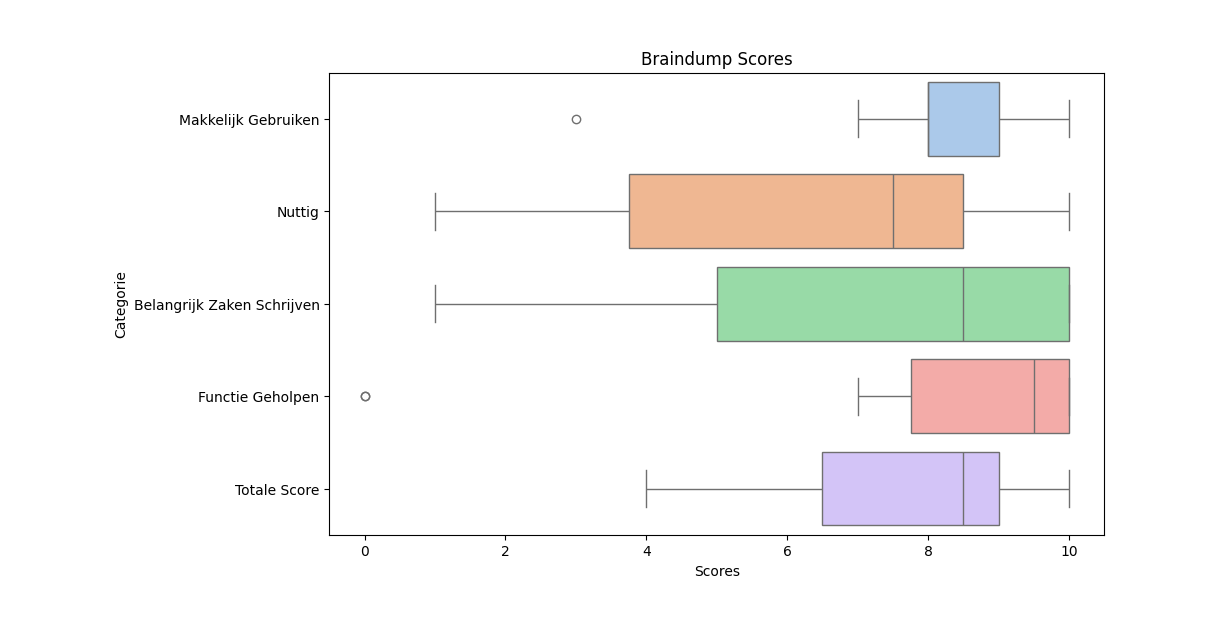
\includegraphics[width=\textwidth]{graphics/data/boxplot_test.png} 
    \caption{Bockplot met resultaten.}
    \label{fig:boxplot_braindump}
\end{figure}

